\section{Fluidodinamica}

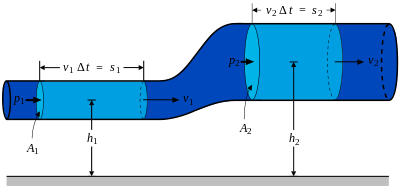
\includegraphics[width=1 \linewidth]{FluidoDinamica/flusso.png} \\

\begin{gather*}
    \textbf{Densità(massa volumica): } \\ \rho = \frac{m}{V} \quad m = \rho V \quad V = \frac{m}{\rho} \\
    \textbf{Pressione: } p = \frac{F_\perp}{S} \\
    \textbf{Pressione Fluidi Comprimibili: } \\ p = p_0e^{-\frac{\rho_0 g}{p_0}z} \\
    \textbf{Pressione atm. ad altitudine $z$: } \\
    p = p_0e^{-\frac{z}{8006km}} \\
    \textbf{Legge di Stevino: } p = \rho g h \\
    \textbf{Principio di Pascal: } \\ p_1 = p_2 \\ \frac{F_1}{S_1} = \frac{F_2}{S_2} \\
    \textbf{Principio di Archimede: } \\ F_A = P_{fl} = m_{fl} g = \rho_{fl} V_{imm} g \\ \begin{cases}
        \rho_{corpo} > \rho_{fluido} & \text{corpo affonda} \\
        \rho_{corpo} < \rho_{fluido} & \text{corpo in equilibrio} \\
        \rho_{corpp} > \rho_{fluido} & \text{corpo galleggia}
    \end{cases} \\
    \textbf{Formula del galleggiamento: } \\ F_A = F_P \\ \rho_{liq} V_{imm} = \rho_{corpo} V_{tot} \\
    \textbf{Portata: } \\ Q = \frac{V}{\Delta t} \\ Q = A \cdot v \\
    \textbf{Teorema di Bernoulli: } \\ p_1 + \frac{1}{2} \rho v_1^2 + \rho g h_1 = p_2 + \frac{1}{2} \rho v_2^2 + \rho g h_2 \\
    \textbf{Equazione di Continuità(ideale): } \\  Q = v_1 S_1 = v_2 S_2 \\
    \textbf{Equazione di Continuità(reale): } \\ Q = \rho_1 v_1 S_1 = \rho_1 v_2 S_2 \\
    \textbf{Velocità 1: } v_1 = \frac{Q}{S_1} = \frac{S_2}{S_1} v_2 \\
    \textbf{Velocità 2: } v_2 = \frac{Q}{S_2} = \frac{S_1}{S_2} v_1 \\
    \textbf{Sezione 1: } S_1 = \frac{v_2}{v_1} S_2 \\
    \textbf{Sezione 2: } S_2 = \frac{v_1}{v_2} S_1 \\\
    \textbf{Differenza di pressione: } \\
    \Delta p = \frac{1}{2} \rho (v_2^2 - v_1^2) \\ 
    \Delta p = \frac{1}{2} \rho (\frac{Q^2}{S_2^2} - \frac{Q^2}{S_1^2})
\end{gather*}